\begin{aufgabe}
	Es sei $G$ eine Gruppe und $E$ ein $G$-Raum, d.h. $E$ ist eine rechts $G$-Menge, so dass die Abbildung $c_g\colon E\to E,\ e\mapsto eg$ stetig ist für alle $g\in G$. Die $G$-Wirkung heißt \emph{frei und eigentlich diskontinuierlich}
	falls jeder Punkt $e\in E$ eine Umgebung $U$ besitzt, so dass
	für alle $g\in G\backslash\{1\}$ gilt, dass $U\cap Ug=\emptyset$.
	Wir bezeichnen mit $E/G$ den Quotientenraum von $E$ nach
	der Äquivalenzrelation $e\sim eg$ für alle $e\in E$ und $g\in G$.	
	\begin{enumerate}[i)]
%		\item Sei $G$ eine endliche Gruppe, die stetig und {\em frei} auf einem
%		Hausdorffraum $E$ wirkt 
%		(d.h. aus $eg=e$ f"ur $e\in E, g\in G$ folgt schon $g=1$). Zeigen Sie,
%		dass die Wirkung von $G$ auf $E$ eigentlich diskontinuierlich ist.
%		%\item Finden Sie eine Gruppe $G$ (notwendigerweise unendlich) und eine
%		%stetige, freie Wirkung von~$G$ auf einem Hausdorffraum, die nicht
%		%eigentlich diskontinuierlich ist.
		\item F"ur jede freie und eigentlich diskontinuierliche Wirkung
		einer Gruppe $G$ auf einem Raum $E$ ist die Quotientenraumprojektion
		\[ E \ \to \ E/G \]
		eine Überlagerung. %Was ist die Blätterzahl?
		\item Sei $E$ ein einfach-zusammenhängender Raum, auf dem eine Gruppe $G$ frei und eigentlich diskontinuierlich wirkt. Für $e\in E$ ist die Fundamentalgruppe $\pi_1(E/G, e)$ isomorph zu $G$. 
		\item Die Wirkung von $\ZZ\rtimes \ZZ$ auf $\R^2$ aus der Vorlesung ist frei und eigentlich diskontinuierlich.
	\end{enumerate}
\end{aufgabe}

\begin{aufgabe}
	Es bezeichne $K= [0,1]\times [0,1] / ((x,0)\sim (x,1)\textup{ und }(0,y) \sim (1, 1-y))$ die Kleinsche Flasche und $T= [0,1] \times [0,1] / ((x,0)\sim (x,1)\textup{ und }(0,y) \sim (1, y))$ den Torus. Da $T\cong S^1\times S^1$ gilt $\pi_1(T,x_0)\cong \ZZ^2$ für jeden Basispunkt $x_0\in T$. 
	\[ 
	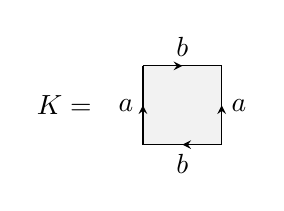
\begin{tikzpicture}[auto, glueing/.style= {->, >=stealth}, scale = 1]
		\node at (-1, 0.5) {$K =$};
		\fill[color = gray!10] (0,0)--(0,1)--(1,1)--(1,0)--(0,0);
		\draw (0,0) to node{$a$} (0,1);\draw[glueing] (0,0) to (0,0.5);
		\draw (1,0) to node[swap]{$a$} (1,1);\draw[glueing] (1,0) to (1,0.5);
		\draw (0,0) to node[swap]{$b$} (1,0);\draw[glueing] (1,0) to (0.5,0);
		\draw (0,1) to node{$b$} (1,1);\draw[glueing] (0,1) to (0.5,1);
	\end{tikzpicture}
	\qquad
	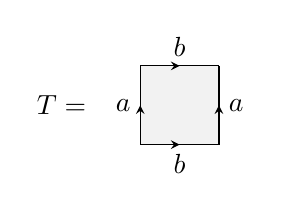
\begin{tikzpicture}[auto, glueing/.style= {->, >=stealth}, scale = 1]
		\node at (-1, 0.5) {$T =$};
		\fill[color = gray!10] (0,0)--(0,1)--(1,1)--(1,0)--(0,0);
		\draw (0,0) to node{$a$} (0,1);\draw[glueing] (0,0) to (0,0.5);
		\draw (1,0) to node[swap]{$a$} (1,1);\draw[glueing] (1,0) to (1,0.5);
		\draw (0,0) to node[swap]{$b$} (1,0);\draw[glueing] (0,0) to (0.5,0);
		\draw (0,1) to node{$b$} (1,1);\draw[glueing] (0,1) to (0.5,1);
	\end{tikzpicture}\]
	Es seien $n, m>0$ zwei ganze Zahlen. Wir betrachten die Teilmenge 
	\[ n\mathbb Z\rtimes m\mathbb Z = \{ ( nk, ml) \mid k,l\in \mathbb Z\} \subset \mathbb Z\rtimes \mathbb Z. \]
	\begin{enumerate}[i)]
		\item $n\mathbb Z\rtimes m\mathbb Z$ ist eine Untergruppe von $\mathbb Z\rtimes \mathbb Z$. Diese ist für $m$ gerade isomorph zu $\mathbb Z\times \mathbb Z$ und für $m$ ungerade isomorph zu $\mathbb Z\rtimes \mathbb Z$.
		\item Konstruiere (notwendigerweise $(n\cdot m)$-blättrige) zusammenhängende Überlagerungen $p_{n,m}\colon T\to K$ für $m$ gerade und $p_{n,m}\colon K\to K$ für $m$ ungerade, sodass die charakteristische Untergruppe in $\pi_1(K, \ast) \cong \mathbb Z\rtimes \mathbb Z$ genau $n\mathbb Z\rtimes m\mathbb Z$ ist.
	\end{enumerate}
	\textbf{Bemerkung:}
		Nicht jede Untergruppe von $\ZZ\rtimes\ZZ$ hat die Form $n\mathbb Z\rtimes m\ZZ$. Jedoch hat jede endliche Überlagerung der Kleinschen Flasche als Totalraum entweder den Torus oder die Kleinsche Flasche selbst, d.h. alle Untergruppen von endlichem Index sind isomorph zu $\ZZ^2$ oder $\ZZ\rtimes\ZZ$.
\end{aufgabe}

\begin{aufgabe}
	Sei $p\colon E\to X$ eine Überlagerung von zusammenhängenden
	und lokal weg-zusammenhängenden Räumen.  Dann sind die folgenden Aussagen äquivalent.
	\begin{enumerate}[i)]
		\item Es gibt ein $x\in X$ so dass die Decktransformationsgruppe $\Delta(p)$
		transitiv auf $p^{-1}(x)$ wirkt.
		\item Für alle $x\in X$ wirkt die Decktransformationsgruppe $\Delta(p)$
		transitiv auf $p^{-1}(x)$.
		\item Es gibt ein $e\in E$ so dass die charakteristische Untergruppe
		$p_*(\pi_1(E,e))$ ein Normalteiler von $\pi_1(X,p(e)))$ ist.
		\item Für alle $e\in E$ ist die charakteristische Untergruppe
		$p_*(\pi_1(E,e))$ ein Normalteiler von $\pi_1(X,p(e)))$.
		\item Die von $p$ induzierte Abbildung
		\[ E/\Delta(p) \ \to \  X\]
		ist ein Homöomorphismus, wobei $E/\Delta(p)$ den
		Quotientenraum von $E$ nach der Wirkung der Decktransformationsgruppe
		bezeichnet.
	\end{enumerate}	
	Wenn diese äquivalenten Bedingungen erfüllt sind, heißt
	die Überlagerung \emph{normal} (oder auch \emph{regulär}).
\end{aufgabe}

\begin{aufgabe}
	Die orientierbare Fläche vom Geschlecht 2 ist folgender Quotient des Oktogons. Berechne die Fundamentalgruppe mit Hilfe des Satzes von Seifert--van Kampen. %Betrachte dazu die im Bild eingezeichnete diagonale Unterteilung und beobachte das beide Seiten Fundamentalgruppe $\ZZ*\ZZ$ haben.
	\[	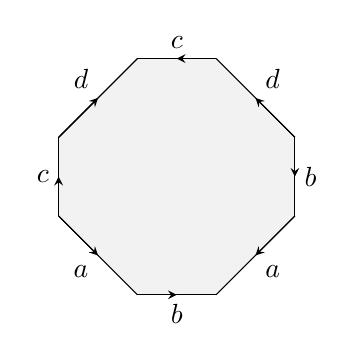
\begin{tikzpicture}[auto, glueing/.style= {->, >=stealth}, scale = 1]
		\fill[color = gray!10] (0,1)--(1,0)--(2,0)--(3,1)--(3,2)--(2,3)--(1,3)--(0,2)--(0,1);
		\draw (0,1) to node[swap]{$a$} (1,0);\draw[glueing] (0,1) to (0.5,0.5);
		\draw (3,1) to node{$a$} (2,0);\draw[glueing] (3,1) to (2.5,0.5);
		\draw (1,0) to node[swap]{$b$} (2,0);\draw[glueing] (1,0) to (1.5,0);
		\draw (3,2) to node{$b$} (3,1);\draw[glueing] (3,2) to (3,1.5);
		\draw (0,1) to node{$c$} (0,2);\draw[glueing] (0,1) to (0,1.5);
		\draw (3,2) to node[swap]{$d$} (2,3);\draw[glueing] (3,2) to (2.5,2.5);
		\draw (0,2) to node{$d$} (1,3);\draw[glueing] (0,2) to (0.5,2.5);
		\draw (2,3) to node[swap]{$c$} (1,3);\draw[glueing] (2,3) to (1.5,3);
		%\draw (0,1) to (3,2);
	\end{tikzpicture}\]
\end{aufgabe}
